\documentclass[border=10pt]{standalone}

\usepackage{tikz}
\usepackage{tikzsymbols}
\usetikzlibrary{calc,patterns,shapes.geometric}

\def\centerarc[#1](#2)(#3:#4:#5){\draw[#1] ($(#2)+({#5*cos(#3)},{#5*sin(#3)})$) arc (#3:#4:#5);}

\begin{document}
	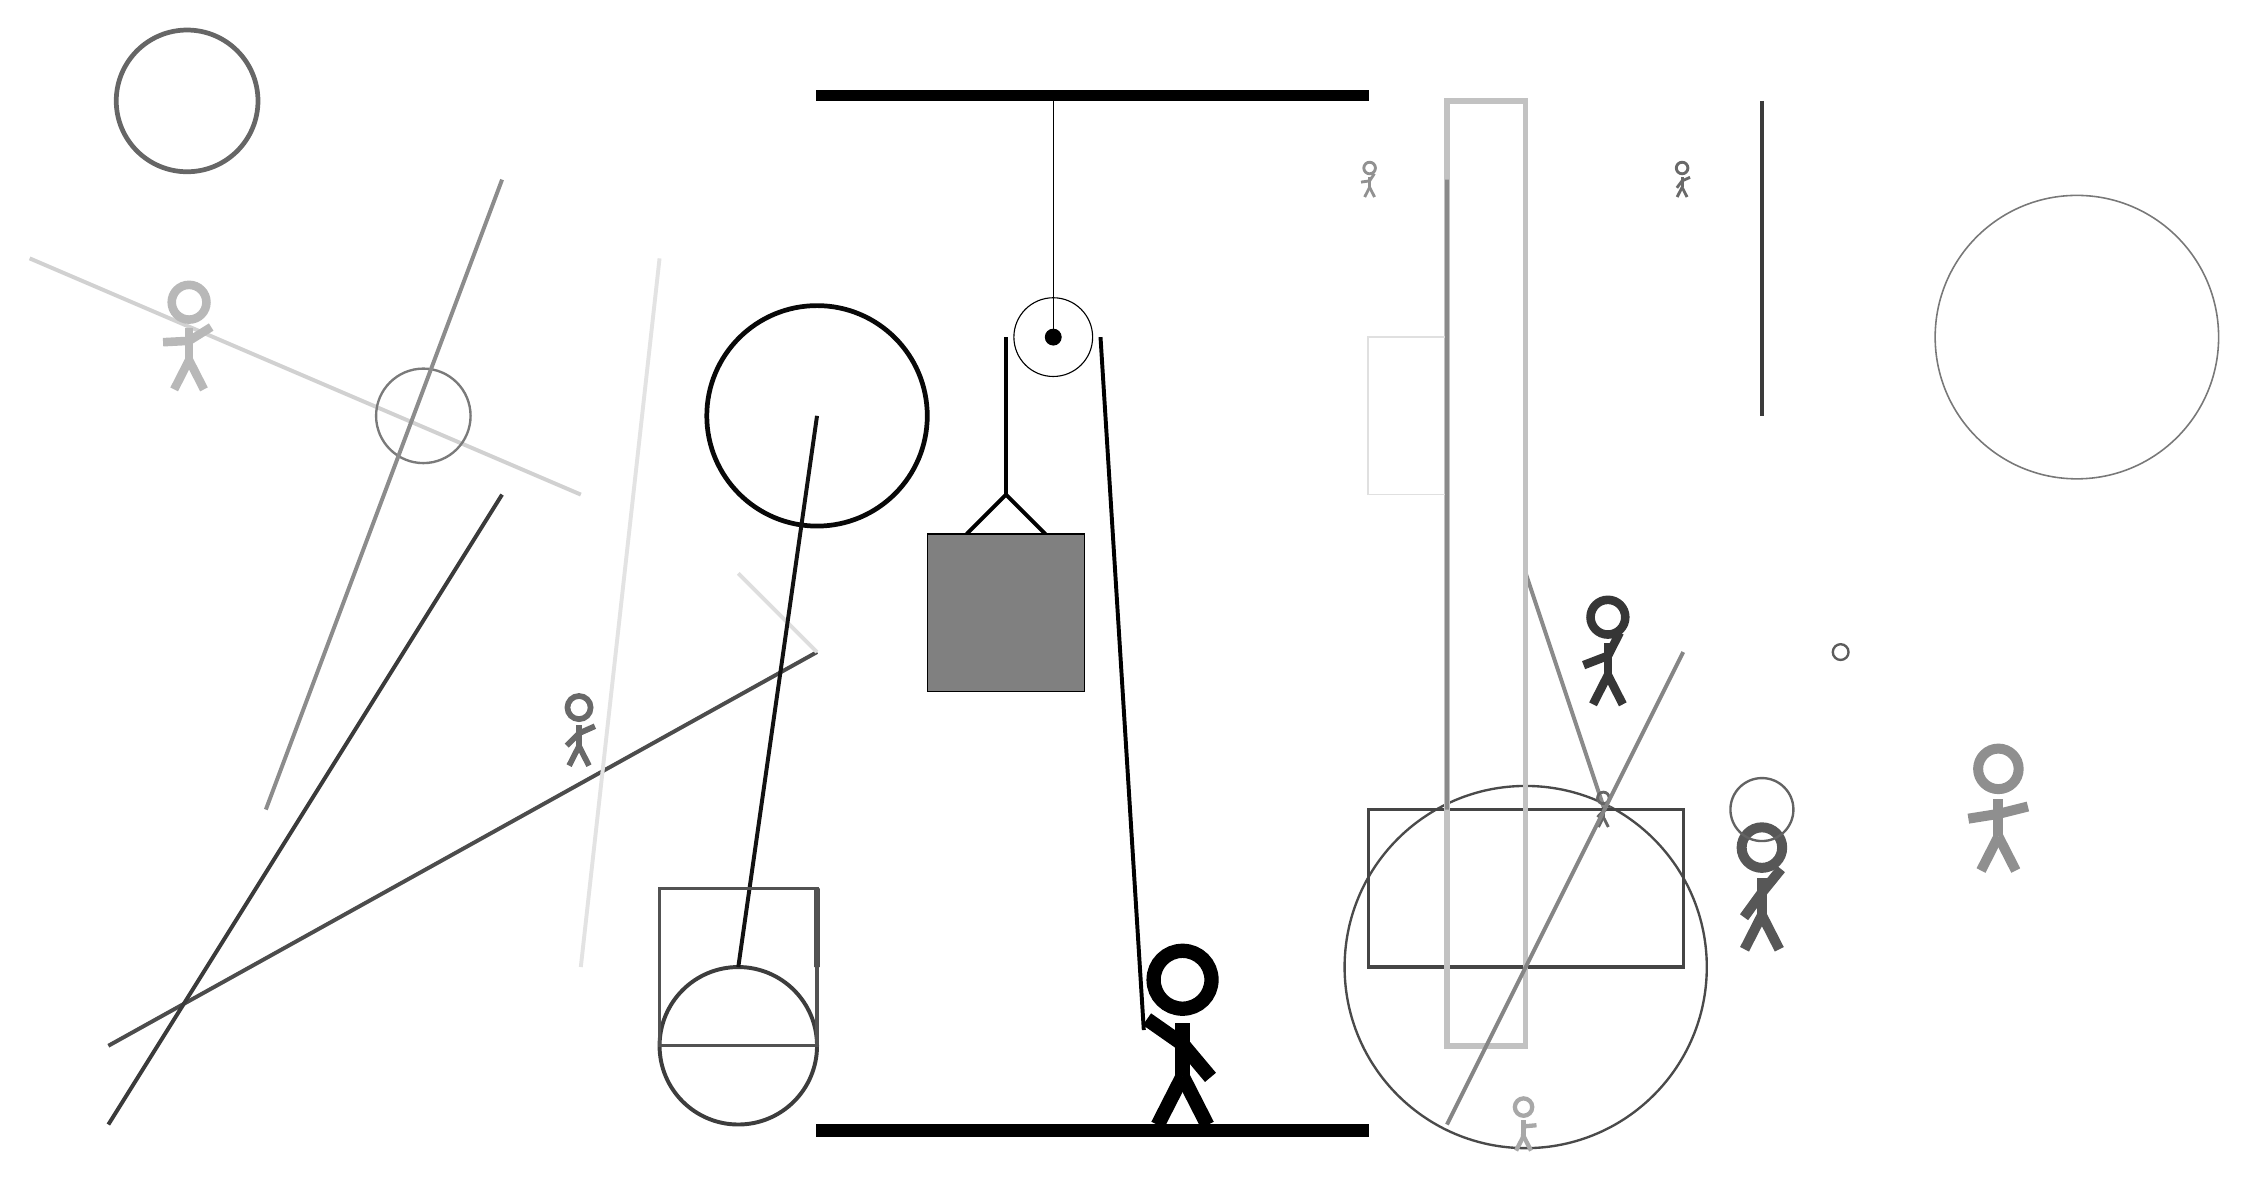
\begin{tikzpicture}
		%%%%% START %%%%%
		
		\draw[fill=black] (-2, 10) rectangle (5, 10.125);
		
		\draw (1, 7) circle (0.5);
		\draw[fill=black] (1, 7) circle (0.1);
		\draw (1, 10) -- (1, 7);
		
		\draw[line width=0.5mm] (-0.1, 4.5) -- (0.4, 5.0) -- (0.9, 4.5);
		\draw[fill=black!50] (-0.6, 4.5) rectangle (1.4, 2.5);
		
		\draw [line width=0.6mm, color=black!60](-10, 10) circle (0.9);
		
		\draw [line width=0.3mm, color=black!71](7, -1) circle (2.3);
		\node[line width=0.7mm, color=black!59] at (-5, 2) {\Strichmaxerl[4][45][24]};
		\draw[line width=0.5mm, color=black!46](7, 4) -- (8, 1);
		
		\node[line width=0.2mm, color=black!66] at (10, 0) {\Strichmaxerl[7][54][51]};
		\node[line width=0.5mm, color=black!60] at (8, 1) {\Strichmaxerl[2][47][22]};
		\draw [line width=0.6mm, color=black!97](-2, 6) circle (1.4);
		\node[line width=0.4mm, color=black!34] at (7, -3) {\Strichmaxerl[3][87][5]};
		\draw [line width=0.5mm, color=black!76](-3, -2) circle (1.0);
		
		\draw[line width=0.5mm, color=black!70](-2, 3) -- (-11, -2);
		\draw[line width=0.4mm, color=black!73] (5, 1) rectangle (9, -1);
		
		\node[line width=0.7mm, color=black!44] at (13, 1) {\Strichmaxerl[7][9][14]};
		\draw [line width=0.3mm, color=black!64](11, 3) circle (0.1);
		\draw[line width=0.7mm, color=black!24] (6, -2) rectangle (7, 10);
		\node[line width=0.7mm, color=black!79] at (8, 3) {\Strichmaxerl[6][21][63]};
		\node[line width=0.4mm, color=black!43] at (5, 9) {\Strichmaxerl[2][8][57]};
		\draw[line width=0.5mm, color=black!13](-3, 4) -- (-2, 3);
		\draw[line width=0.5mm, color=black!18](-5, 5) -- (-12, 8);
		\node[line width=0.3mm, color=black!59] at (9, 9) {\Strichmaxerl[2][53][24]};
		
		\draw [line width=0.2mm, color=black!53](14, 7) circle (1.8);
		\node[line width=0.4mm, color=black!28] at (-10, 7) {\Strichmaxerl[6][3][32]};
		\draw[line width=0.5mm, color=black!48](9, 3) -- (6, -3);
		
		\draw[line width=0.5mm, color=black!93](-3, -1) -- (-2, 6);
		\draw[line width=0.5mm, color=black!77](10, 10) -- (10, 6);
		\draw[line width=0.7mm, color=black!69] (-2, 0) rectangle (-2, -1);
		
		\draw [line width=0.3mm, color=black!52](-7, 6) circle (0.6);
		\draw[line width=0.5mm, color=black!45](-6, 9) -- (-9, 1);
		\draw[line width=0.2mm, color=black!12] (6, 5) rectangle (5, 7);
		\draw [line width=0.3mm, color=black!61](10, 1) circle (0.4);
		
		\draw[line width=0.5mm, color=black!77](-6, 5) -- (-11, -3);
		\draw[line width=0.4mm, color=black!46] (6, 1) rectangle (6, 9);
		
		\draw[line width=0.4mm, color=black!68] (-2, -2) rectangle (-4, 0);
		\draw[line width=0.5mm, color=black!11](-4, 8) -- (-5, -1);
		\draw [line width=0.6mm, color=black!99](-8, 0) circle (0.0);
		
		\draw[line width=0.5mm] (0.4, 7) -- (0.4, 5.0);
		\centerarc[line width=0.5mm](1, 7)(0:180:0.6);
		\draw[line width=0.5mm](1.6, 7) -- (2.15, -1.8);
		
		\node at (2.6, -1.9) {\Strichmaxerl[10][-35][-50]};
		
		\draw[fill=black] (-2, -3) rectangle (5, -3.15);
		
		%%%%% END %%%%%
	\end{tikzpicture}
\end{document}